%Introduction

\section{Introduction}
American National Standards Association (ANSI) defines the Circuit Breaker (CB) as, \textquotedblleft A mechanical switching device, capable of making, carrying, and breaking currents under normal circuit conditions and also making, carrying for a specified time, and breaking currents under specified abnormal circuit conditions such as those of short circuit\textquotedblright
 \cite{DefinitionforPower}. CBs are required to fulfil following physical requirements apart from main functions \cite{van2001transients}.

\begin{itemize}
\item Should work as a good conductor when closed and a good insulator when opened
\item Should quickly interrupt the short circuit current
\item Should not generate over voltages during switching
\item Should be highly reliable during operation
\end{itemize}

Components involved in basic functions of High Voltage Circuit Breakers (HVCBs) can be divided into five groups \cite{cigre2000user}.

\justify
\begin{description}[style=nextline, before={\setcounter{descriptcount}{0}},font=\bfseries\stepcounter{descriptcount}\thedescriptcount.~]

\item[Contacts] Contacts are the main component which should be able to carry the rated current continuously without overheating and should carry large current without welding for a short period during short circuit condition. Hence contacts are the key component in deciding the success or failure of the CB. Condition monitoring of contacts avoids the failure of this critical component.

\item[Switching] CBs are subjected to electrical, thermal and mechanical stresses during switching. It is required that CBs should be able to perform its duty under normal and abnormal conditions without causing failure. The parameters like pole mismatch, contact travel, contact wear, operating time and arcing time are used to monitor the switching of CB. 

\item[Insulation] The insulating components must be so designed as to withstand the mechanical and electrical stresses. In HVCBs solid, liquid, vacuum and gaseous dielectric materials are used to provide electrical insulation.

\item[Operating Mechanism] The function of the operating mechanism is to open and close the circuit breaker contacts within the specified limits. CBs remain in closed position for an extended period of time. But during fault condition, it has to open reliably. Hence the job of the operating mechanism is not simple. The percentage of failure of operating mechanism is large in the total failures of HVCBs.

\item[Control and auxiliary functions] Control and auxiliary components are controlled by 110-220 V DC. According to reliability surveys, control and auxiliary components are exposed to failures relatively frequently. Delay in operation or failing to open or close on demand are some typical failures in these parts.
\end{description}

\setlength{\parskip}{1em}

Renewable energy sources are being used to cater the power demand in the fast growing power systems. The reliable switching of CBs in controlling power flows and during critical contingency condition is important \cite{hedman2009optimal, kezunovic2014reliable, gu2014fast}. CBs gets deteriorated due to usage and ageing. Hence they need proper maintenance. Conventionally CBs have been maintained through time-based maintenance schedule \cite{hinow2011substation, li2004cost, razi2013priority, liu2010optimal, razi2013priorityassessment}.

In POWERGRID network failure survey was carried out. Since the CB operation is~ not~ frequent~ for~ extra high~ voltage network, manufacturers~ recommend overhauling of CB after ten years of service or at a specific number of operations. It was observed that there had been damages in the components in the interrupting chambers much before ten years where as there were few CBs with 17-20 years of age in good condition with no abnormality \cite{sodha2012condition}. Thus condition based maintenance has been reported as the most efficient to recognize the need for maintenance of CBs when necessary. It is the cost effective maintenance and ensures the reliability \cite{long2012online, gungor2012cognitive, moghe2012smart, razi2014circuit, qiang2012high}.

CIGRE has conducted three world wide surveys since 1970 on high voltage CBs reliability \cite{janssen2014international,mazza1981first,cigre1994final,cigre2012final}. The reliability is expressed in failure per 100 CB years (CBY) or per 10,000 operating cycles for the relevant failure modes. Failures are classified as a major failure (MaF or MF) and minor failures (Mf or Mif). The third enquiry included CBs of all ages and the objective was the relationship between age and major failure rate. Figure \ref{fig:Application of CBs} shows that 54\% of the total population is for the overhead line.

\begin{figure}[!htbp]
    \centering
    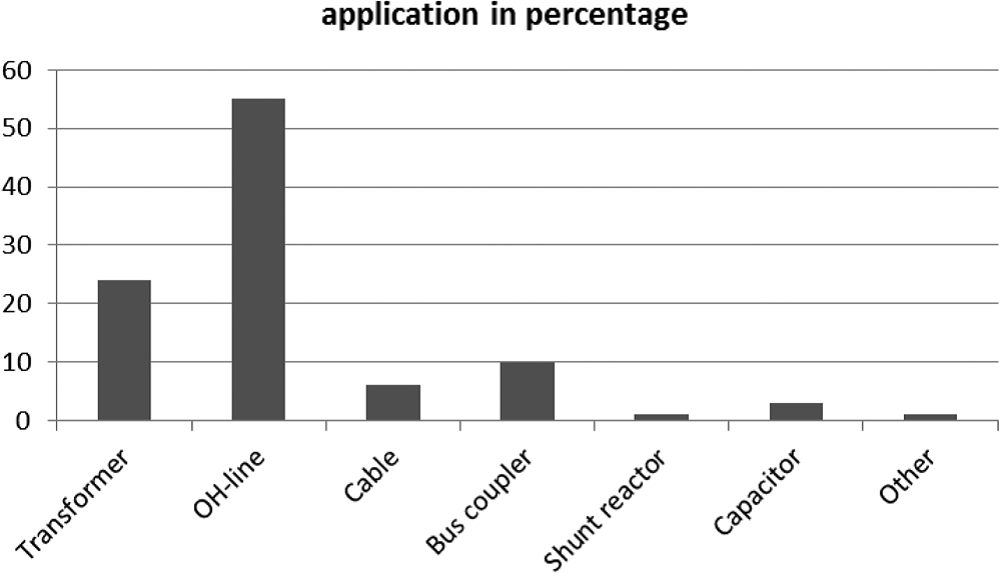
\includegraphics[width=\textwidth]{ApplicationofCBs}
    \caption[Application of CBs]{Application of CBs \cite{janssen2014international}}
    \label{fig:Application of CBs}
\end{figure}

Shunt reactors and shunt capacitor bank percentage is very less, but they cover more than 20\% of failure. The technology of operating mechanism is changing towards spring mechanism as seen in figure \ref{fig:Maf Rate per Drive Technology for Failures [18]}. Table \ref{table:Percentage of Maf Rate} shows the percentage of MaF and MiF rate per failure mode reported in the third enquiry.

\begin{figure}[!htbp]
    \centering
    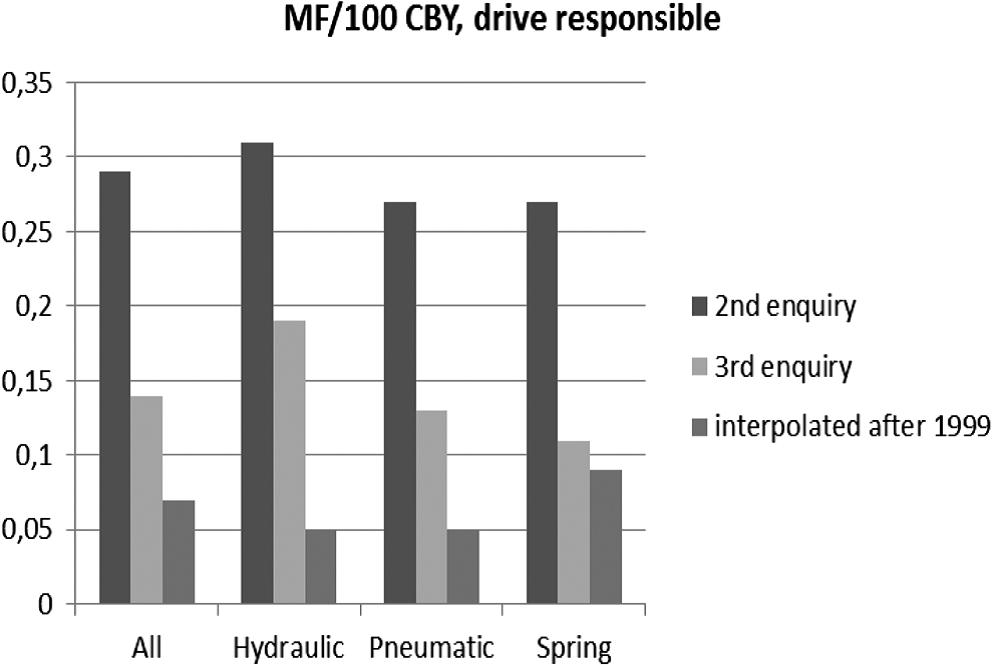
\includegraphics[width=\textwidth]{MafRateper}
    \caption[Maf-Rate per Drive Technology for Failures]{Maf-Rate per Drive Technology for Failures \cite{janssen2014international}}
    \label{fig:Maf Rate per Drive Technology for Failures [18]}
\end{figure}


\begin{table}[!htbp]
\begin{threeparttable}
\renewcommand{\arraystretch}{1.3}
\caption{Percentage of Maf Rate and Mif Rate per Failure Mode, Third Inquiry}
\label{table:Percentage of Maf Rate}
\centering
\small
\begin{tabular}{| >{\arraybackslash}m{1.9in} |>{\centering\arraybackslash}m{0.6in} |>{\arraybackslash}m{3in} |}

%\begin{tabular}{| l | c | l |}
\hline
\multicolumn{1}{|c|}{\textbf{MaF failure mode}}	&	\textbf{MaF(\%)}	& \multicolumn{1}{|c|}{\textbf{Comments}}								\\ \hline
Does not close on command	&	28.2				& Mainly with live tank circuit breakers			\\ \hline
Does not open on command	&	16.4				&													\\ \hline
Closes without command		&	0.2					&													\\ \hline
Opens without command		&	5.4					&													\\ \hline
Fails to carry the current	&	1.3					&													\\ \hline
Dielectric breakdown		&9.9					& Breakdown to earth: 5\%, Internal breakdown across open pole, during opening operation = does not break the current: 1.9\%, Other across open pole: 1.8\%, Breakdown between poles: 1.2\%					\\ \hline
Locked in open or closed position & 25.1			& Alarm has been triggered by the control system	\\ \hline
Loss of mechanical integrity&	8.1					& Mechanical damage of parts						\\ \hline
Other						&	5.2					&													\\ \hline
Total						&	100					&													\\ \hline \hline
\multicolumn{1}{|c|}{\textbf{MiF failure mode}}	& \textbf{Mif(\%)}		& \multicolumn{1}{|c|}{\textbf{Comments}}									\\ \hline
Air or hydraulic oil leakage&	20.3				& In operating mechanism							\\ \hline
Small SF\textsubscript{6} gas leakage		& 35.6					& Large leakage will give MF-mode \textquotedblleft
Locked\textquotedblright
			\\ \hline
Oil leakage in grading capacitors &	1.0				&													\\ \hline
Change in functional characteristics& 28.4			& 6.8\% mechanical; 3.3\% electrical 18.3\% control%
													  and auxiliary systems								\\ \hline
Other and no answer			& 14.6					&													\\ \hline
Total						& 100					&													\\ \hline
\end{tabular}
%\begin{tablenotes}
%\item \cmark -- functionality is available. \hspace{0.5in} \xmark -- functionality is not available.
%\end{tablenotes}
\end{threeparttable}
\end{table}

\subsection{Circuit Breaker Classification}
Figure \ref{Fig:Classification of CBs} shows the complete classification of circuit breakers. However, CBs are classified mainly according to the dielectric medium used for arc extinguishing \cite{nasrallah2007electrical}.

\begin{sidewaysfigure}
   \centering 
   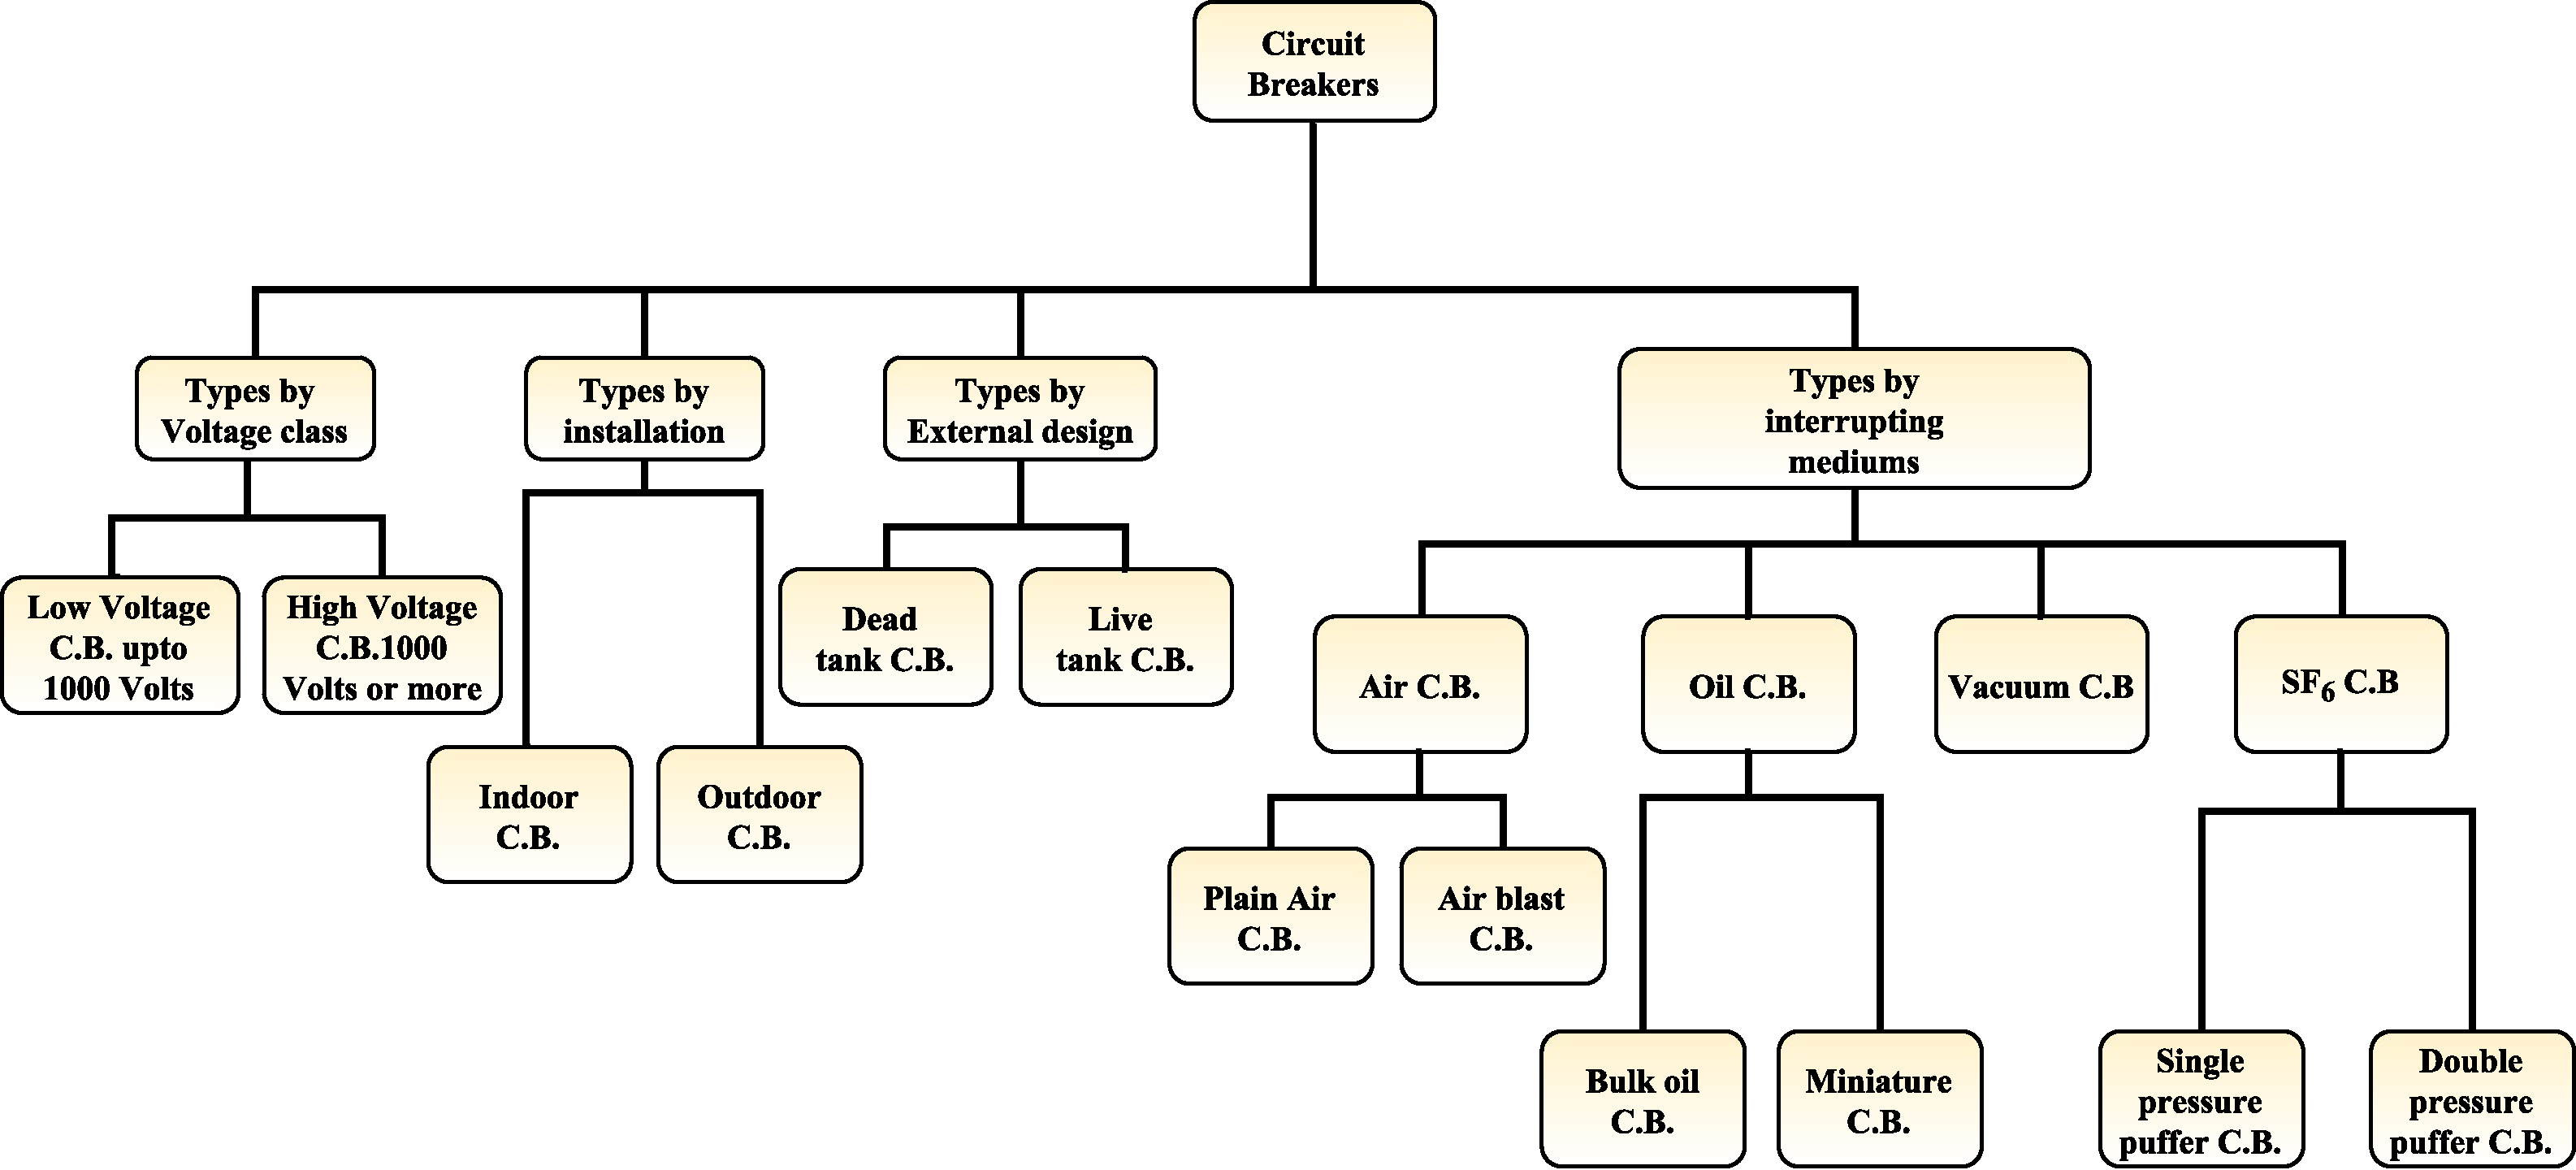
\includegraphics[width=\textwidth]{ClassificationofCBs} 
   \caption{Classification of CBs}
   \label{Fig:Classification of CBs}
\end{sidewaysfigure}

\clearpage
\section{Motivation}
The power system is growing at a faster pace. Increase in level of transmission voltage necessitates the use of HVCBs. The reliability of system depends on the CBs which has a crucial role in isolating the faults. Most of the population of circuit breakers in high voltage transmission is SF\textsubscript{6} circuit breakers. Modern high voltage puffer type SF\textsubscript{6} circuit breakers have two parallel contact sets. The low resistance silver plated main contacts carry the load current whereas the tungsten-
copper arcing contacts, which opens after the main contact are exposed to arcing. Hence arcing contacts are liable to damage due to severe thermal stresses and Transient Recovery Voltage (TRV). Damaged main and arcing contacts reduce the short circuit capacity of the circuit breaker. Therefore the condition assessment of circuit breakers contact is of prime importance.

Study of CB failures survey by CIGRE working group observed that the failures are mainly due to malfunction of the operating mechanism and control circuit. The major contribution of the fault is from aging, wear and corrosion (50\%) followed by the manufacturing faults, design faults and incorrect maintenance (15\%) \cite{janssen2014international}. Failure survey motivated to study circuit breaker condition monitoring aspects.

\clearpage
\section{Objectives}
The objectives of the proposed research work are, to:
\begin{enumerate}
\item  Study the interruption of current under three phase to ground terminal fault at the substation for multiple line switching and transformer switching and to measure the TRV and compare it with standard TRV to determine the short circuit capability of the CB

\item Study the interruption of single phase to ground short line fault and to measure the TRV and compare it with standard TRV to determine the short circuit capability of the CB

\item Measure and study~ the static contact resistance~ and~ dynamic~ contact resistance of 245 kV and 400 kV SF\textsubscript{6} CBs at the High Voltage circuit breaker manufacturing industry and in the field

\item Collect the data of DCRM for normal and abnormal cases from the PGCIL, MSETCL and High Voltage  circuit breaker manufacturing industry

\item Analyze the DCRM data and develop an algorithm to determine the wearing of main and arcing contacts, contact wipe to determine the health of CB

\item Apply the Black Box Cassie - Mayer arc model for arc interruption studies
\end{enumerate}

\clearpage
\section{Theme}
The interruption chamber of circuit breaker comprises of sets of the fixed and moving main and arcing contacts which are prone to erosion with time and usage. The lack of direct access to those and use of high-pressure gas complicate the direct condition assessment of this part. Circuit breakers need to perform various switching duties. Switching under the different fault condition and certain normal duty leads to severe TRVs across the contacts of the circuit breakers which may fail the circuit breaker to clear the fault and has the influence on the short circuit capacity of the circuit breaker. Hence the main theme of the proposed work has been to study the TRV under different fault conditions for IEEE network and determine the short circuit capability of the breaker using computer simulations in EMTP-RV. Also to measure the dynamic contact resistance of circuit breaker using the 4-wire method by injecting 100 A DC through the breaker. Measurements are recorded with a resolution of 100 $\mu s$ with a sampling frequency of 100 kHz. Figure \ref{fig:Theme of the Research Work} shows the theme of the research work and Figure \ref{fig:Normal DCRM Signature} indicates the DCRM signature. Measurements are done in the field and industry. Measured data and collected data from Power Grid Corporation of India Ltd. (PGCIL), Maharashtra State Electricity Transmission Company Ltd. (MSETCL) and High Voltage circuit breaker manufacturing industry have been analyzed in detail using HISAC Ultima test manager software. Results of analysis and simulations carried out are presented leading to conclusions and finally to new contributions. A new algorithm has been proposed to detect the contact anomaly. A computer program is developed in Java to determine the health of CB.


\begin{figure}[!htbp]
    \centering
    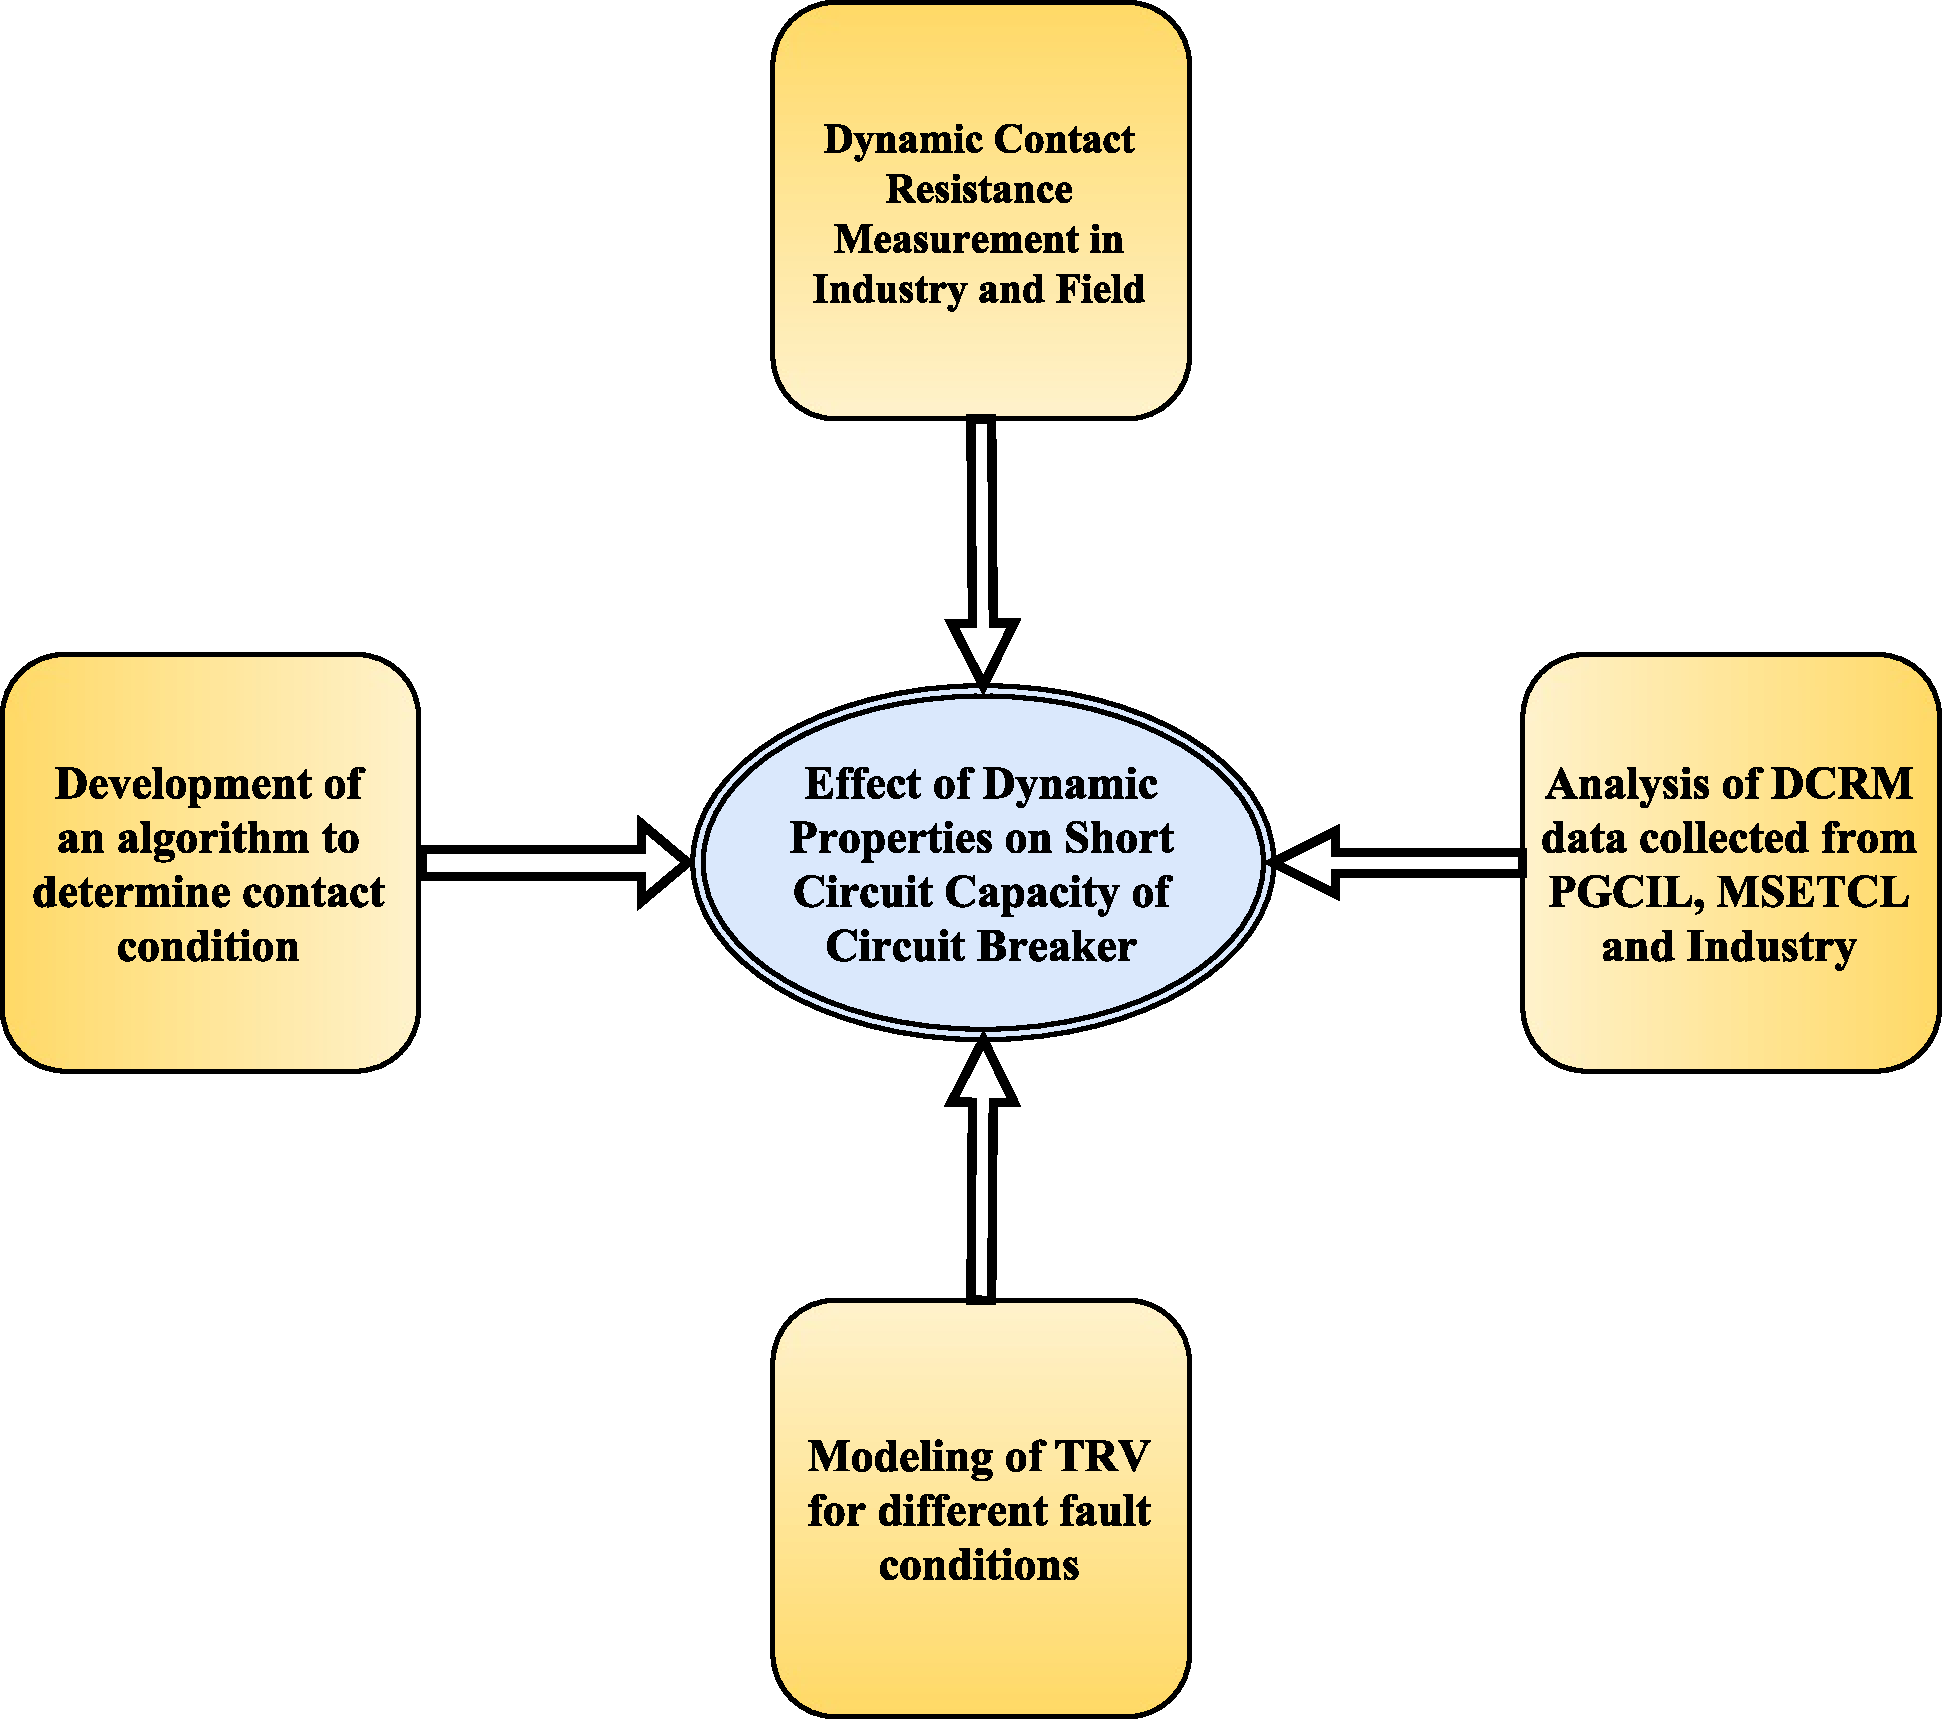
\includegraphics[width=\textwidth]{ThemeoftheResearchWork}
    \caption{Theme of the Research Work}
    \label{fig:Theme of the Research Work}
\end{figure}

\begin{figure}[!htbp]
    \centering
    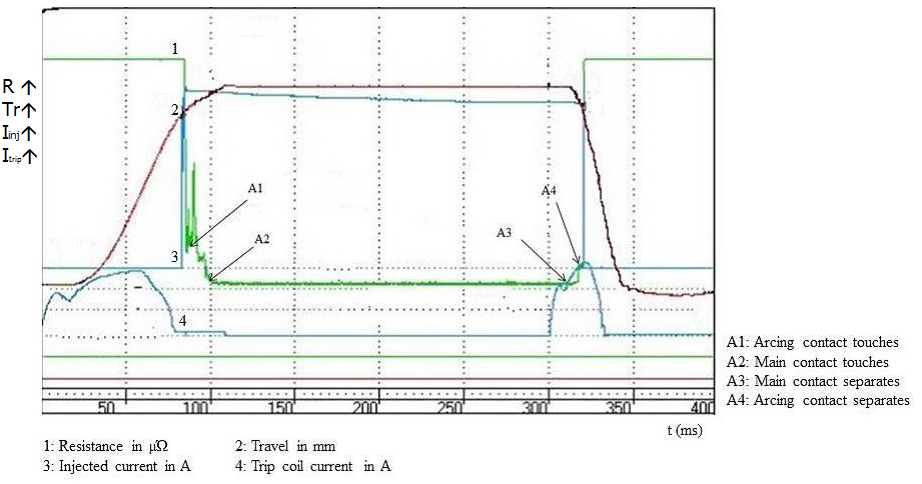
\includegraphics[width=\textwidth]{NormalDCRMSignature}
    \caption{Normal DCRM Signature}
    \label{fig:Normal DCRM Signature}
\end{figure}

\setlength{\parskip}{0em}
\clearpage
\section{Organization} 
The thesis is organized in following interdependent parts with a continuous theme as per abstract.
\subsubsection*{Chapter 1} Introduction - This chapter addresses the aspects containing introductory part. The necessity and the objectives of this research work are clearly mentioned. The overall theme of the complete research work is presented.
\subsubsection*{Chapter 2} Literature Survey - A summary of the exhaustive literature survey is represented. An overview of arc modeling, Transient Recovery Voltage, Dynamic Contact Resistance Measurement (DCRM), Standards related to circuit breaker timings are discussed in detail.
\subsubsection*{Chapter 3} System Development - Computational model of IEEE network for TRV study under different fault conditions is developed in EMTP-RV. Similarly analytical and mathematical models are developed. Dynamic contact resistance measurement is explained. Mathematical treatment is explained in detail with relevant references.
\subsubsection*{Chapter 4} Performance Analysis - Results of analytical and computational methods are presented. Justification for difference is given. Measured and collected data of DCRM from field is analyzed in detail using HISAC ULTIMA test manager software and new algorithm is proposed to detect the contact anomaly. Computer program in Java is developed to determine the health of circuit breaker.
\subsubsection*{Chapter 5} Conclusions - In this chapter conclusions of the research work, future work and  applications are presented.